% This LaTeX was auto-generated from MATLAB code.
% To make changes, update the MATLAB code and export to LaTeX again.

\documentclass{article}

\usepackage[utf8]{inputenc}
\usepackage[T1]{fontenc}
\usepackage{lmodern}
\usepackage{graphicx}
\usepackage{color}
\usepackage{hyperref}
\usepackage{amsmath}
\usepackage{amsfonts}
\usepackage{epstopdf}
\usepackage[table]{xcolor}
\usepackage{matlab}
\usepackage[active,tightpage]{preview}

\renewcommand{\PreviewBorder}{1in}
\newcommand{\Newpage}{\end{preview}\begin{preview}}

\sloppy
\epstopdfsetup{outdir=./}
\graphicspath{ {./ecen415_images/} }

\begin{document}
\begin{preview}

\matlabheading{Section A - Formative Questions}

\begin{par}
\begin{flushleft}
1. Consider the example in the notes where we regulated the continuous time system that had 
\end{flushleft}
\end{par}

\begin{par}
\begin{flushleft}
$\mathit{\mathbf{A}}=\left\lbrack \begin{array}{ccc}
0 & 1 & 0\\
0 & 0 & 1\\
-18 & -15 & -2
\end{array}\right\rbrack$, and so forth.
\end{flushleft}
\end{par}

\begin{par}
\begin{flushleft}
(a) [10 marks] Build another regulator for this system, this time implementing your controller in discrete time.
\end{flushleft}
\end{par}

\begin{par}
\begin{flushleft}
Notes: You should try to make your controller more or less the same as the continuous time version, but you don’t need to make it exactly the same.
\end{flushleft}
\end{par}

\begin{par}
\begin{flushleft}
You will need to make a discrete time model of the plant and are free to choose an appropriate sampling time. Don’t choose a sampling time that is too fast, because that will make the system behaviour too similar to the continuous time system and and will make the exercise dull.
\end{flushleft}
\end{par}

\begin{matlabcode}
clc; clear;

%% State space system model
A = [0, 1, 0;
     0, 0, 1;
     -18, -15, -2];
B = [0;
     0;
     1];
C = [1, 0, 0];
D = 0;

% Pole Placement in continuious time
p = [-1.33+1.49j, -1.33-1.49j, -13.3];
K = place(A,B,p);

% Select the sampling time
ts = 1/5;

%% create both the open and closed loop systems
sys = c2d(ss(A, B, C, D), ts);
sys_ctrl = c2d(ss(A-B*K, B, C, D), ts);

%% Impulse Figure

figure
impulse(sys)
hold on 
impulse(sys_ctrl)
legend("Open Loop", "Closed Loop")
hold off
\end{matlabcode}
\begin{center}
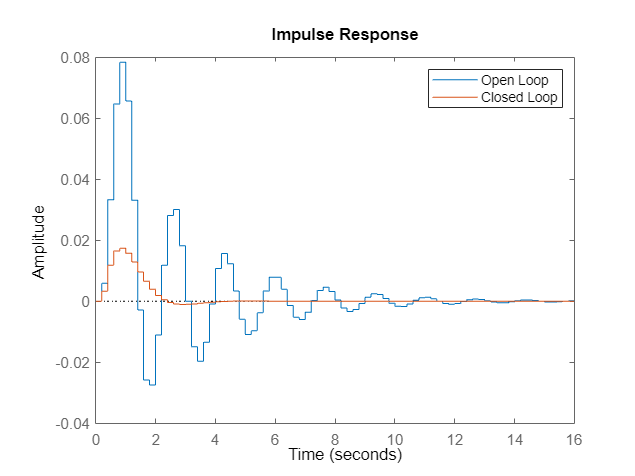
\includegraphics[width=\maxwidth{57.90265930757652em}]{figure_0.png}
\end{center}

\hrule

\matlabheading{Section B - Summative Questions}




\begin{matlabcode}
%% Set up the state space model
clear; clc;

A = [-10,   0,  -90, 295, -205,    0;
       0, -50,  -50, 125, -375, 1000;
       0,   0, -100, 200, -300,  500;
       0,   0, -500, 100,  200,  500;
       0,   0,  500,-300,- 400,  500;
       0,   0,    0,-250, -250, -200];

B = [1, 0;
     0, 2;
     0, 0;
     0, 0;
     0, 0;
     0, 0];

C = [1,1,-2,0,0,0];

D = [0, 0];

sys = ss(A, B, C, D);
\end{matlabcode}

\hrule
\matlabheading{Question a)}


\vspace{1em}
\begin{par}
\begin{flushleft}
The system is not controllable, as the rank of it's controllability matrix is not equal to the rank of the A matrix.
\end{flushleft}
\end{par}

\begin{par}
\begin{flushleft}
By placing the system in the \textbf{modal canonical form}, the $A$ matrix has it's eigenvalues (system poles) arranged along its diagonal. From this form we can directly see from the $B$ matrix which system poles can be effected by the input, and are therefore controllable. 
\end{flushleft}
\end{par}

\begin{par}
\begin{flushleft}
It can be seen that $\lambda_1 \;\textrm{and}\;\lambda_2$ are controllable, while $\lambda_3 \;\lambda_4 \;\lambda_5 \;\textrm{and}\;\lambda_6$ are not controllable.
\end{flushleft}
\end{par}

\begin{par}
\begin{flushleft}
From the \textbf{modal canonical }$A$ matrix it can also be seen that the system is stabilisable, as all of the uncontrollable poles wjithin this system are stable.
\end{flushleft}
\end{par}


\vspace{1em}
\begin{matlabcode}
if rank(ctrb(A, B)) ~= rank(A)
    fprintf("Controlability matrix is not full rank, system is
             uncontrollable")
end
\end{matlabcode}
\begin{matlaboutput}
Controlability matrix is not full rank, system is uncontrollable
\end{matlaboutput}
\begin{matlabcode}
csys = canon(sys, 'modal');
csys.A
\end{matlabcode}
\begin{matlaboutput}
ans = 6x6    
  -10.0000         0         0         0         0         0
         0  -50.0000         0         0         0         0
         0         0 -100.0000  500.0000         0         0
         0         0 -500.0000 -100.0000         0         0
         0         0         0         0 -200.0000  500.0000
         0         0         0         0 -500.0000 -200.0000

\end{matlaboutput}
\begin{matlabcode}
csys.B
\end{matlabcode}
\begin{matlaboutput}
ans = 6x2    
     2     0
     0     2
     0     0
     0     0
     0     0
     0     0

\end{matlaboutput}


\vspace{1em}

\hrule
\matlabheading{Question b) }


\vspace{1em}
\begin{par}
\begin{flushleft}
The slowest uncontrollable modes are $\lambda_3 \;\textrm{and}\;\lambda_4 \to s=-100\pm 500j$. Because of this we will look to plave the two controllable poles at locations greater than -100. 
\end{flushleft}
\end{par}

\begin{matlabcode}
%% Remove the uncontrollable state variabled from the modal form
A_ctrl = [-10, 0;
           0 ,-50];

B_ctrl = [1, 0;
          0, 2];

C_ctrl = [1,1];

D = [0, 0];

%% Place the poles beyond the slowest pole at s = 100
K = place(A_ctrl, B_ctrl, [-110, -150]);

sys_model_ctrl = ss(A_ctrl - B_ctrl*K, B_ctrl, C_ctrl, D);

%% Plot the controlled system without uncontrollable states
figure
impulse(sys_model_ctrl)
title("Impulse Response of Controlled Simplified Model")
\end{matlabcode}
\begin{center}
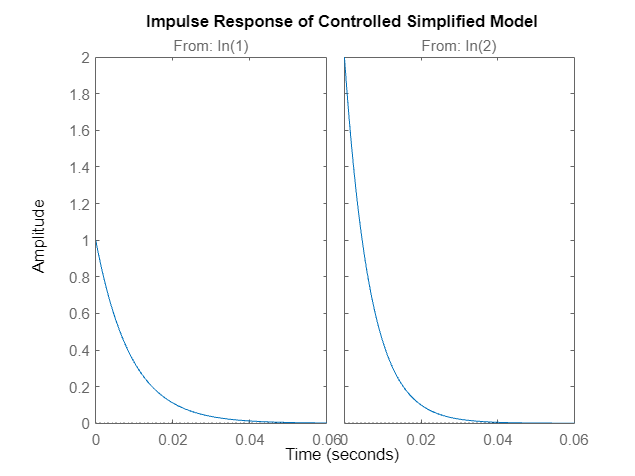
\includegraphics[width=\maxwidth{57.90265930757652em}]{figure_1.png}
\end{center}

\begin{par}
\begin{flushleft}
This figure shows the impulse of the newly controlled simplified model.
\end{flushleft}
\end{par}

\begin{matlabcode}
%% Place the poles within the full system with the uncontrolled states
K = place(A, B, [-110, -150, -100-500j, -100+500j, -200-500j, -200+500j]);
sys_ctrl = ss(A - B*K, B, C, D);

figure
impulse(sys);
hold on
impulse(sys_model_ctrl);
h = impulseplot(sys_ctrl);

p = getoptions(h);
p.XLim = {[0, 0.6]; [0, 0.15]};
title("Impulse Responses")
legend('Open Loop', 'Simplified Model', 'Complete Closed Loop')
setoptions(h, p);
hold off
\end{matlabcode}
\begin{center}
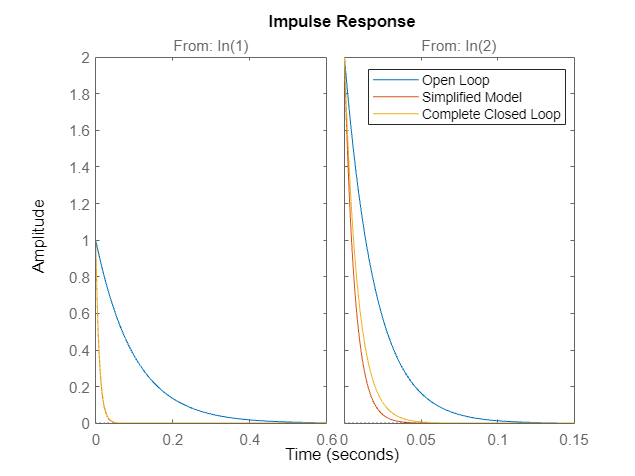
\includegraphics[width=\maxwidth{57.90265930757652em}]{figure_2.png}
\end{center}

\begin{par}
\begin{flushleft}
From the above plot it can be seen that the impulse response of the simplified model and the full system model are quite similar. It can also be seen that they both offer a large speed increase of the original system
\end{flushleft}
\end{par}

\hrule
\matlabheading{Question c)}

\begin{matlabcode}
%% Set up the integrator state space model
A_i = [A, zeros(length(A), 2);
       -1, 0, 0, 0, 0, 0, 0, 0;  % This integrator looks at the first input
       0, -1, 0, 0, 0, 0, 0, 0]; % This integrator looks at the second input

B_i = [B; 0, 0; 0, 0];

C_i = [C, 0, 0];

%% Place the new integrator poles
K_i = place(A_i, B_i, [-110, -150, -100-500j, -100+500j, 
                       -200-500j, -200+500j, -200, -200]);

sys_i = ss(A_i - B_i * K_i, [zeros(length(B), 2);1, 0; 0, 1], C_i, D);


figure
h = stepplot(sys);
hold on
step(sys_model_ctrl);
step(sys_i);
p = getoptions(h);
p.yLim = {[0, 1.2]};
setoptions(h, p);
legend("Open Loop", "Initial Regulator", "Integral Control");
hold off
\end{matlabcode}
\begin{center}
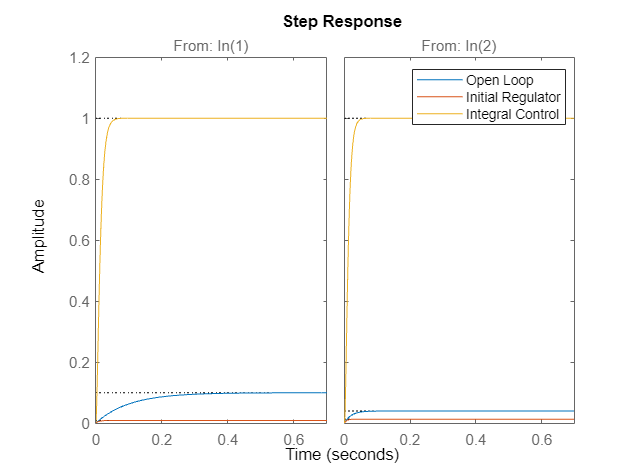
\includegraphics[width=\maxwidth{57.90265930757652em}]{figure_3.png}
\end{center}

\begin{par}
\begin{flushleft}
It can be seen that the addition of intergrators to the system completly removes the steady state error of perviously designed regualtor. 
\end{flushleft}
\end{par}

\begin{matlabcode}
A_perturbed = A_i;
A_perturbed(1,1)=-1;
A_perturbed(1,2)=50;
A_perturbed(2,1)=-25;
sys_p = ss(A_perturbed - B_i * K_i, [zeros(length(B), 2);1, 0; 0, 1], C_i, D);

figure
h = stepplot(sys_i);
hold on
step(sys_p);
p = getoptions(h);
p.yLim = {[0, 1.2]};
setoptions(h, p);
legend("Initial A Matrix", "Perturbed A Matrix");
hold off
\end{matlabcode}
\begin{center}
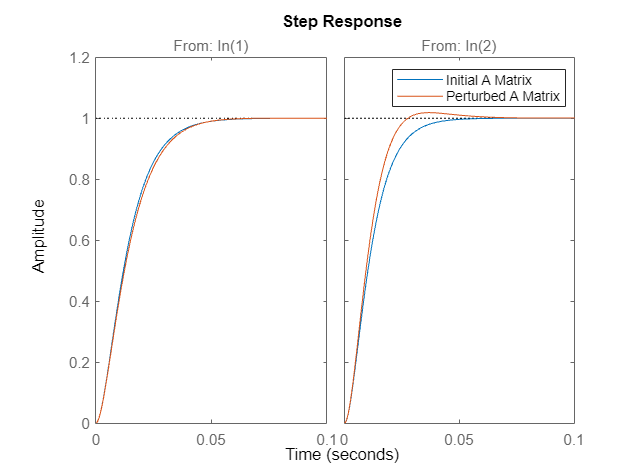
\includegraphics[width=\maxwidth{57.90265930757652em}]{figure_4.png}
\end{center}

\begin{par}
\begin{flushleft}
The system was perturbed by modifying the $A$ matrix values, and adding new values. From the plot above we can see that the controlled system is resilient to inaccuracies in the system model. 
\end{flushleft}
\end{par}

\hrule
\matlabheading{Question d)}

\begin{matlabcode}
x_0 = [0.1, 0.5, 0, 1, 1, 0.5, 0, 0];

t = 0:0.5/10000:0.5;
u = zeros(length(t), 2);

u(t > 0.1, 1) = 1; % Input 1, step of 1
u(t > 0.2, 2) = 1; % Input 2, step of 1
u(t > 0.3, 1) = 0; % Input 1, step of 0
u(t > 0.4, 2) = 0; % Input 2, step of 0

figure
[y, t, x] = lsim(sys_i, u, t, x_0);
hold on
plot(t, y);
plot(t, u(1:end,1), '-', 'color',[.6 .6 .6], 'LineWidth',2)
plot(t, u(1:end,2), '--', 'color',[.6 .6 .6], 'LineWidth',2)
ylim([-0.75, 2.05]);
legend("Output", "u_1", "u_2")
title("Linear Simulaton Results")
ylabel('Amplitude');
xlabel('time (seconds)');
grid on
box on
hold off
\end{matlabcode}
\begin{center}
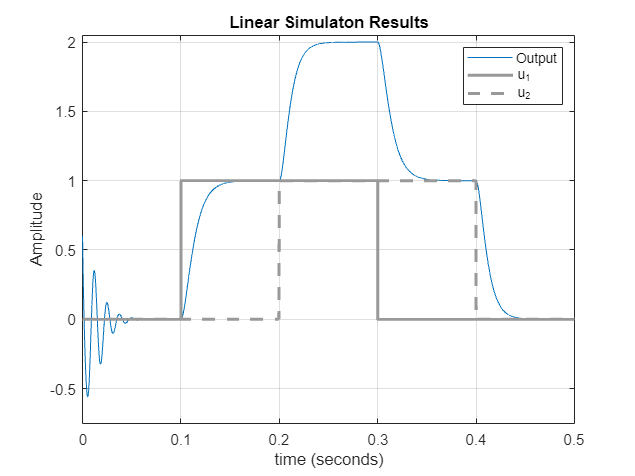
\includegraphics[width=\maxwidth{57.90265930757652em}]{figure_5.png}
\end{center}

\end{preview}
\end{document}
